After having explained the research work and summarized the necessary theory preliminaries in the previous chapters, this chapter goes through the steps of modeling the prosumer-based direct current microgrid with iterative learning control. Section \ref{sec:networkmodel} starts off with the \textit{low voltage direct current microgrid dynamics} (\ref{subsec:prod_cons_model}), followed by the definition of the \textit{prosumer-based direct current microgrid model} (\ref{subsec:prosumer}). The following section \ref{sec:ilc} derives the \textit{structure and design of the iterative learning controller}, by defining the \textit{control objectives} (\ref{subsec:conobj}), the structure of the \textit{higher-layer controller} (\ref{subsec:hlc}) and the \textit{learning dynamics} (\ref{subsec:learndyn}).

\section{Network model of the prosumer-based DC microgrid with lower-layer control}
\label{sec:networkmodel}
In this section, we model the network of the prosumer-based DC microgrid and define the dynamics of it. The model is adapted by the \textit{low voltage direct current microgrid} dynamics, proposed by Lia Strenge in her master thesis \cite{lia_master}, where a distinction is made between producers and consumers. In this thesis, however, the model and equations are adapted to combine producer and consumer as prosumer. Despite everything it is necessary to be introduced to these dynamics, to have a better understanding for the modeling in Section \ref{subsec:prosumermodel}

\subsection{Network modeling of the producer-consumer DC microgrid}
\label{subsec:prod_cons_model}
This Section serves as a base and defines the equations, that inspired the prosumer-based microgrid network dynamics and the lower-layer controller, respectively, with no influence of the ILC. We assume a constant demand for the consumer nodes and no higher-layer control input, to make the derivation of the equations clearer. \\
As explained above, the modeling of this network topology and the definitions and equations mentioned in this Section are proposed by Lia Strenge in "\textit{Modeling and simulation of a droop controlled swarm
type low voltage DC microgrid in a DAE framework - Master Thesis}" \cite{lia_master}, as well as the work "\textit{Stability of meshed DC microgrids using
probabilistic analysis}" by L. Strenge, H. Kirchhoff, G.L. Ndow and F. Hellmann \cite{lia_stability}.
\\ Recall from \ref{sec:power_network}, that a microgrid is considered as an \textit{undirected graph}. Then $N \in \mathbb{N}$ is the number of producers and consumers. The grid nodes $gn \in \{1,2,...,N\} =: \mathcal{N} \subset \mathbb{N}$ with = $\mathcal{N} = \mathcal{N}_P \cup \mathcal{N}_C$ represent the producers $n_P \in \mathcal{N}_P$ with index $j = 1,...,n_P$  and consumers $n_C \in \mathcal{N}_C$ with index $k = n_P+1,...,N$ and $n_P + n_C = N$, while the edges $pl \in \{1,2,...,m\} =: \mathcal{M} \subset \mathbb{N}$ with $m \leq N(N-1)/2$ and the index $jk$, represent the power lines connecting the producers with the consumers. 
\\ The network is modeled as an undirected connected graph with the edge-vertice-incidence matrix $\boldsymbol{M} \in \mathbb{R}^{m \times N }$, see (Eq. \ref{equation:incidence_def}) in Section \ref{sec:power_network}. Since the network is electric, the Kirchhoff laws must hold. The currents sum to zero at each node (Kirchhoff current law) and the voltages sum to zero in each mesh (kirchhoff voltage law) \cite{lia_master}. With these laws, we obtain the equations \cite{lia_master}:
\setlength{\abovedisplayskip}{5pt}
\setlength{\belowdisplayskip}{5pt}
\setlength{\abovedisplayshortskip}{0pt}
\setlength{\belowdisplayshortskip}{0pt}
\begin{align}
    v_{pl}(t) &= \boldsymbol{M}v_{gn}(t) \label{eq:incv} \\
    i_{gn}(t) &= \boldsymbol{M}i_{pl}(t) \label{eq:inci}
\end{align}
where $t \in \mathbb{R}$ is the time in seconds, $\boldsymbol{M} \in \mathbb{R}^{m \times N}$ is the incidence matrix of the network; $v_{pl}(t) = (v_{pl,1}(t),...,v_{pl,m}(t))^T: \mathbb{R} \rightarrow \mathbb{R}^m$ is the vector of power line voltages in volt or the voltage difference between the connected grid nodes, respectively; $v_{gn}(t) = (v_{1}(t),...,v_{N}(t))^T: \mathbb{R} \rightarrow \mathbb{R}^N$ is the vector of grid node voltages in volt; $i_{gn}(t) = (i_{1}(t),...,i_{N}(t))^T: \mathbb{R} \rightarrow \mathbb{R}^N$ is the vector of the currents sum at the grid nodes in ampere and $i_{pl}(t) =(i_{pl,1}(t),...,i_{pl,m}(t))^T: \mathbb{R} \rightarrow \mathbb{R}^m$ is the vector of the power line currents in ampere \cite{lia_master}. \\Furthermore, we make the following assumptions:
\begin{enumerate}[i.]
    \item Every node can feed electricity into the microgrid (producer with $i_{to,grid,j}(t) > 0, j = 1,...,n_P$), receive from the microgrid (consumer with $i_{to,grid,k}(t) < 0, k = n_P+1,...,N$) \cite{lia_stability} 
    \item At each node, there is no other information available other than local variables. Hence, the control is fully decentralized.
    \item The generation current at the producer nodes is known with \cite{lia_stability}
    \begin{align}
        i_{gen,j}(t) = K_{D,j}(V_{ref,j} - v_j(t)) \label{eq:i_gen}
    \end{align} where $K_{D,j} > 0$ is the voltage droop coefficient and $V_{ref,j}$ the reference voltage at producer node $j \in \mathcal{N}_P$. Droop control (with its according droop coefficient mathimatically) is applied in a microgrid to stabilize the voltage drop \cite{voltage_droop}. 
    \item The current to the load at the consumer nodes is assumed to be known with \cite{lia_stability}
    \begin{align}
        i_{load,k}(t) = \frac{P_k(t)}{v_k(t)}, v_k(t) \neq 0 \label{eq:i_load}
    \end{align} where $P_k$ is the load power drawn from the grid at consumer node $k \in \mathcal{N}_C$. 
    \item \label{ass:induct} A power line in low voltage direct current applications behaves mostly inductive \cite[p.28]{lia_master} with the context
    \begin{align}
        L_{pl,jk} \frac{di_{pl,jk}(t)}{dt} = v_{pl,jk}(t)-R_{pl,jk}i_{pl,jk}(t) \label{eq:induct}
    \end{align} where $L_{pl,jk}$ is the known inductance, $R_{pl,jk}$ the known resistance, $i_{pl,jk}(t)$ the power line current and $v_{pl,jk}(t)$ the power line voltage at power line $jk \in \mathcal{M}$. Since current flows in both directions, we further assume $L_{pl,jk} = L_{pl,kj}$, $R_{pl,jk} = R_{pl,kj}$, and $i_{pl,jk}(t) = i_{pl,kj}(t)$
    \item \label{item:cap} A producer or consumer can be electrically modeled by a current source, represented by the equation (Eq. \ref{cap_eq}) and a capacitor in parallel as in (Eq. \ref{cap_i}) \cite{lia_master}. 
    \begin{align}
        i_{gn}(t) &= f(t,q) - i_{cap}(t) \label{cap_eq}\\
        i_{cap}(t) &= \boldsymbol{C_{cap}}\frac{dv_{gn}(t)}{dt} \label{cap_i}
    \end{align}
    with $f: \mathbb{R}\times \{0,1\}^N \rightarrow \mathbb{R}^N$ as a source current vector in Ampere, $i_{cap}(t) = (i_{cap,1}(t),...,i_{cap,2}(t))^T: \mathbb{R} \rightarrow \mathbb{R}^N_{>0}$ as a vector of capacitor currents in Ampere and $\boldsymbol{C_{cap}} = \diag{(C_{cap,1},...,C_{cap,N})}^T \in \mathbb{R}^{N \times N}_{>0}$ as diagonal matrix of capacitances in Farad \cite{lia_master}.
\end{enumerate}
In assumption \ref{item:cap}. the source current vector can be distinguished between the generation current from (Eq. \ref{eq:i_gen}) and the load current from (Eq. \ref{eq:i_load}) with 
\begin{align}
    f(t,q) =\begin{cases}
K_{D,j}(V_{ref,j} - v_j(t)),& i_{to grid,i}(t) >0\\
\frac{P_k(t)}{v_k(t)}, & \, i_{to grid,i}(t) <0
\end{cases} \label{eq:fallunterscheidung_strom}
\end{align}
with $i = 1,...,n$ as the considered node and $v_k(t) \neq 0$. Furthermore we assume that the load power is constant, $P_k(t) = P, P \in \mathbb{R}$ Combining equations (Eq. \ref{eq:fallunterscheidung_strom}), (Eq. \ref{cap_eq}) and (Eq. \ref{cap_i}) and distinguishing between producer and consumer grid node voltage with 
\begin{align}
    v_{gn}(t) = \left[\begin{array}{c} v_P(t) \\ v_C(t) \end{array}\right] 
\end{align}
producers listed first ($v_P(t) = (v_1(t),...,v_{n_P}(t))^T$) and consumers listed last ($v_C(t) = (v_{n_P+1}(t),...,v_n(t))^T$), we get the following equation \cite{lia_stability}:
\begin{align}
    \boldsymbol{C_{cap}}\left[\begin{array}{c} \frac{dv_P(t)}{dt} \\ \frac{dv_C(t)}{dt} \end{array}\right] = -i_{gn}(t) + \left[\begin{array}{c} \boldsymbol{K_{D}}(V_{ref,P} - v_P(t)) \\ P/v_C(t) \end{array}\right]
\end{align}
$i_{gn}(t) = (i_{gn,1}(t),...,i_{gn,N}(t))^T: \mathbb{R} \rightarrow \mathbb{R}^N$ is the vector of the currents sum at the grid nodes in ampere; $\boldsymbol{K_D} = \diag(K_{D,j})$ is the diagonal droop coefficient matrix, $j$ the producer index, as above; $V_{ref,P} = (V_{ref,1},...,V_{ref,n_P})^T$ the vector of the reference node voltages of the producers; $P = (P_1,...,P_{n_c})^T$ is the load power vector of the consumers \cite{lia_stability}. \\From equation (Eq. \ref{eq:induct}) in assumption \ref{ass:induct} we get the equation: 
\begin{align}
    \boldsymbol{L_{pl}} \frac{di_{pl}(t)}{dt} = v_{pl}(t)-\boldsymbol{R_{pl}}i_{pl}(t) 
\end{align} in vector representation, with $\boldsymbol{L_{pl}} = \diag(L_{pl,jk})$ the diagonal power line inductance matrix and $\boldsymbol{R_{pl}} = \diag(R_{pl,jk})$ the diagonal power line resistance matrix \cite{lia_stability}. Recall, that $v_{pl}(t) = (v_{pl,1}(t),...,v_{pl,m}(t))^T: \mathbb{R} \rightarrow \mathbb{R}^m$ is the vector of power line voltages in volt or the voltage difference between the connected grid nodes.
\\With (Eq. \ref{eq:inci}) and (Eq. \ref{eq:incv}) we obtain the model equation system (Eq. \ref{eq:1}) and (Eq. \ref{eq:2}) in matrix vector form \cite{lia_stability}
\begin{align}
    \boldsymbol{L_{pl}} \frac{di_{pl}(t)}{dt} &= \boldsymbol{M}v_{gn}(t)-\boldsymbol{R_{pl}}i_{pl}(t) \label{eq:1} \\
    \boldsymbol{C_{cap}}\left[\begin{array}{c} \frac{dv_P(t)}{dt} \\ \frac{dv_C(t)}{dt} \end{array}\right] &= -\boldsymbol{M}i_{pl}(t) + \left[\begin{array}{c} \boldsymbol{K_{D}}(V_{ref,P} - v_P(t)) \\ P/v_C(t) \end{array}\right] \label{eq:2}
\end{align}
The overall producer-consumer direct current microgrid model is shown in Figure
 \ref{fig:prod-cons-micro}. 
%\label{subsec:prodconsmodel}
\begin{figure}[h]
\centering
    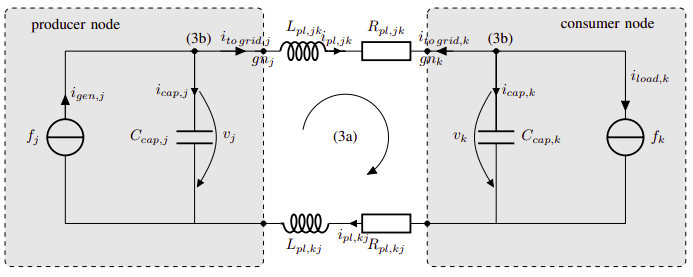
\includegraphics[scale=0.5]{pictures/prod-cons-microgrid.png}
    \caption{Model for the direct current microgrid. Here, simplified for $n = 2$ nodes and time argument $(t)$. Index $j$ for producers, index $k$ for consumers. $i_{gen,j}(t) = f_{j}(t)$ are droop controlled sources (Eq. \ref{eq:i_gen}), $i_{load,k}(t) = f_k(t)$ are constant power load (Eq. \ref{eq:i_load}) \cite{lia_stability}}
    \label{fig:prod-cons-micro}
\end{figure}
Based on this system we can now define the network model of the prosumer-based structured microgrid in the next Section.
Note that the load power is only in this Section considered as constant. Also, there is no higher-layer control input. For the purpose of the iterative learning control we must assume in the next Section that the power demand has a periodic and fluctuating character. 
\subsection{Network model of the prosumer-based DC microgrid with lower-layer control}
\label{subsec:prosumermodel}
\begin{figure}[h]
	\centering
	\caption{Model for the proposed prosumer-based direct current microgrid. Here, simplified for $n = 2$ nodes.}
	\label{fig:pros-micro}
\end{figure}
Based on the network modeled in Section \ref{subsec:prod_cons_model}, the slightly different prosumer-based direct current model can be derived in this Section. Additionally the low-level control input is going to be used as well as the high-level control input, since the low-layer control structure must be considered now. It is also now going to be assumed, that the load profiles have periodic components in contrast to Section \ref{subsec:prod_cons_model}. \\
In Section \ref{subsec:prosumer}, it is considered that a node in a prosumer-based dirrent current microgrid can feed power into the microgrid, receive power from it or not participate in the microgrid, see Definition \ref{prosumer_def}. Therefore there is no differentiation anymore between producer and consumer; A node must be modeled as one unit combined by the two at first seperate units. 
\\Recall Figure \ref{fig:prod-cons-micro}, where the model for the direct current, non-prosumer-based microgrid is illustrated. The seperate producer $j$ node is connected via the power line $jk$ with the consumer node $k$. For the prosumer-based model, this schema can be adapted, but the power line $jk$ connects prosumer $j$ with prosumer $k$, respectively. Furthermore, $N \in \mathcal{N}$ is the number of prosumers. Therefore, the grid node voltages are now defined as \\$v_gn(t) = (v_1(t),...,v_n(t))^T$.
Obviously, the node structure needs to be changed, so it can produce but also consume simultaneously.
\\A suggestion for this idea would be to combine the generation and load unit into one node. This means that a prosumer in the network is a \textit{parallel connection} of the generation current source and the load current source. As in system (\ref{eq:fallunterscheidung_strom}) the generated and load current remain for a prosumer $j$ in a microgrid and $t \in \mathbb{R}$ as follows: 
\setlength{\abovedisplayskip}{5pt}
\setlength{\belowdisplayskip}{5pt}
\setlength{\abovedisplayshortskip}{0pt}
\setlength{\belowdisplayshortskip}{0pt}
\begin{align}
i_{gen}(t) &= K_{D,j}(V_{ref,j} - v_j(t)) \label{eq:igen}\\
i_{load}(t) &= \frac{P^d_j(t)}{v_j(t)} \label{iload}
\end{align}
For the control, the demand power $P_j(t)$ will be the uncontrolled net power demand $P_j^d(t) = P_j^f(t) + P_j^p(t)$ at node $j$ which
accounts for the actual demand or uncontrollable infeed
from renewable sources \cite{paperilc}. It consists of a fluctuating part $P_j^f(t)$ and a 
and a periodic part $P_j^p(t)$ whose period is empirically
known/estimated \cite{paperilc}, $t \in \mathbb{R}$. 
\\ The model of the power line can be defined as in assumption \ref{ass:induct} (\ref{subsec:prod_cons_model}) in (Eq.\ref{eq:induct}) with 
\begin{align*}
L_{pl,jk} \frac{di_{pl,jk}(t)}{dt} = v_{pl,jk}(t)-R_{pl,jk}i_{pl,jk}(t)
\end{align*}
The prosumers have the same behavior as explained in assumption \ref{item:cap} in Section \ref{subsec:prod_cons_model} and can be modeled by a current source and load. A current source for the higher-layer control input is added parallel to the generating current source. The ILC current is derived from the high-level control input $u^{ILC}$ (Section \ref{subsec:hlc})with:
\begin{align}
i_{ILC,j}(t) = \frac{\boldsymbol{u}^{ILC}_j(t)}{v_j(t)}, v_j(t)\neq 0
\end{align}  For this we need to consider Figure \ref{fig:pros-micro} and the Kirchhoff current law, which led to the following equation:
\begin{align}
C_{cap,j}\frac{dv_j(t)}{dt} &= i_{ILC,j}(t) + i_{gen,j}(t) - i_{j}(t) - i_{load,j}(t) \nonumber \\
C_{cap,j}\frac{dv_j(t)}{dt} &= \frac{\boldsymbol{u}^{ILC}_j(t)}{v_j(t)}+ K_{D}(V_{ref,j} - v_j(t)) - i_{j}(t) - \frac{P^d_j(t)}{v_j(t)} \label{eq:1_pros}
\end{align}
(Eq. \ref{eq:1_pros}) can be derived using (Eq. \ref{eq:igen}) and (Eq. \ref{iload})
\\For the inherent ODE formulation of (\ref{eq:1_pros}) and (Eq.\ref{eq:induct}) , we obtain the closed-loop equations


\begin{subequations}\label{eq:system}
	\begin{empheq}{align}
	\boldsymbol{L_{pl}} \frac{di_{pl}(t)}{dt} &= \boldsymbol{M}v_{gn}(t)-\boldsymbol{R_{pl}}i_{pl}(t)
	\\
	\boldsymbol{C_{cap}}\frac{dv_{gn}(t)}{dt} &= \frac{\boldsymbol{u}^{ILC}(t) - P^d(t)}{v_{gn}(t)} + \boldsymbol{\ K_{D}}(V_{ref} - v_{gn}(t)) -\boldsymbol{M}i_{pl}(t), t \in \mathbb{R}
	\end{empheq}
\end{subequations}
with $P^d(t) = (P^d_1(t),...,P^d_n(t))$ being the vector of the uncontrolled net power demand, consisting of a fluctuating part $P^f(t) = (P^f_1(t),...,P^f_n(t))$ and a periodic part $P^p(t) = (P^p_1(t),...,P^p_n(t))$.
\\To achieve bounded voltage deviation from the reference voltage of the grid in the lower layer of the control architecture, we use a first order controller that we refer to as the lower-layer control. The control law is given as: 
\begin{align}
\boldsymbol{u}^{LI} = \underbrace{\boldsymbol{K_{D}}(V_{ref} - v_{gn}(t))}_{i_{gen}(t)} \cdot v_{gn}(t) \label{eq:ll_energy}
\end{align}

\section{Higher-layer controller structure and design}
\label{sec:ilc_design}
Recall that in this work the control consists of two layers, the low-level controller, see Section \ref{subsec:prosumermodel} and the high-level control. The low-level controller is responsible for the bounded voltage deviation and the power sharing. 
\\In this Section the iterative learning controller is going to be, based on the provided information in Section \ref{subsec:ilc} and the "\textit{Iterative learning control in prosumer-based microgrids with hierarchical control}" paper \cite{paperilc} introduced and modeled. The \textit{control objectives} are derived in Section \ref{subsec:conobj}, and based on the next Section \ref{subsec:hlc} the \textit{higher-layer controller} is designed. 
\subsection{Control objectives}
\label{subsec:conobj}
The proposed overall control objectives are derived in \cite{paperilc} and \cite{lia_master} and combined. 
\begin{enumerate}[(1)]
	\item \label{enum:bounded_voltage} Bounded voltage deviation from the reference voltage of the grid, i.e., \cite{lia_master}.
	\begin{align}
	|v_{gn,j}(t)-V_{ref,j}| &\leq e_V, \forall t \in \mathbb{R}, j \in \mathcal{N}, e_V \in \mathbb{R}_{>0}
	\end{align}
	\item \label{enum:power_sharing} Power sharing of the prosumers \cite{lia_master}: The same amount of power is fed from all of the prosumers into the grid when the time deriatives are zero \cite{lia_master}.
	\begin{align}
	\lim_{t\rightarrow \infty} P_{gn,j}(t) = \lim_{t\rightarrow \infty} P_{gn,k}(t), j,k\in\mathcal{N}
	\end{align}
	\item \label{enum:llc_small} Low-level control energy small \cite{paperilc}: 
	\begin{align}
	\sum_{h=1}^{24} || \textbf{y}^{c,h}||_2 = \sum_{h=1}^{24} || \int_{t^c_h}^{t^c_{h+1}} \textbf{u}^{LI}(\tau) d\tau ||_2 \ll \sum_{h=1}^{24} ||\textbf{u}^{c,h}||_2, c \in \mathbb{N}_0, h=1,...,24
	\end{align} 
\end{enumerate}
(\ref{enum:bounded_voltage}) is achieved through the low-level control regardless of the additional higher-layer control input as long as $|\sum_{j\in \mathcal{N}}u^{ILC}-P^d_j| \leq |\sum_{j\in \mathcal{N}}P^d_j|$ \cite{paperilc}. In the next Section the scheme of the higher-layer controller is designed. In this work, an iterative learning controller is used for this purpose, proposed by Lia Strenge et al. in \cite{paperilc}
\subsection{Iterative learning controller}
\label{subsec:hlc}
Recall (Eq. \ref{eq:ilc_inp_th}). The new input is designed so that the new error is smaller than the previous input. The proposed ILC approach and its parameters by \cite{paperilc} learns a power infeed that compensates the periodic demand component. With $c \in \mathbb{N}_0$ and $h=1,...,24$, with $c$ being the cycle with a duration of one day and $h$ the hour, the following learning input is implemented: 
\begin{align}
\label{eq:control_ilc}
\textbf{u}^c = \textbf{Q}(\textbf{u}^{c-1} - \textbf{Ly}^{c-1}), c > 0
\end{align}
The daily input $\textbf{u}^c$ is adjusted based on the error that is the low-level control energy of the previous day $\textbf{y}^{c-1}$. The desired low-level control energy is zero. $\textbf{L} \in \mathbb{R}^{24N\times 24N}$ is the learning matrix, which is simply chosen to be $\textbf{L}(\kappa) = \kappa I$ with a single scalar parameter $\kappa \in \mathbb{R}_{>0}$ and $\textbf{Q}$ is a butterworth low-pass filter with a relative cutoff frequency of $f_c = 1/6$ \cite{paperilc}. 
\\The proposed ILC approach can reduce the lower-layer control energy, since the required should be zero by learning the periodic demand \cite{paperilc}.
\\The overall proposed nonlinear model with iterative learning control (\ref{eq:system}), (\ref{eq:ll_energy}) and (\ref{eq:control_ilc}) shall be validated, simulated and analyzed under certain assumptions in the next Chapter.

